\section{Introduction}

\subsection{Motivation}
While running in electron-positron collision mode at a center-of-mass energy of \SI{240}{\giga\electronvolt}, the Future Circular Collider is expected to produce on the order of $10^6$ events of the Higgs-strahlung process $\Pep\Pem\to\PZ\PH$. Studying the kinematics of this process allows for the probing of CP-violation at the $\PH\PZ\PZ^*$ vertex. The fractional CP-odd coupling of the $\PH$ boson to two $\PZ$ bosons can be defined as $$f^{\PH\PZ\PZ}_{CP} = \frac{|a^{\PH\PZ\PZ}_3|^2}{\Sigma |a^{\PH\PZ\PZ}_i|^2(\sigma^{\PH\PZ\PZ}_i/\sigma^{\PH\PZ\PZ}_3)}$$

In the first-order $q^2-$expansion of the effective Lagrangian from which the above expression is derived, the $a_i$ can be treated as  constants corresponding to dimension-six operators. In particular, $a_3$ characterizes the strength of CP-odd interactions at the $\PH\PZ\PZ$ vertex. The values $\sigma_i$ correspond to the effective cross section of the $\PH\to\PZ\PZ$ decay process with $a_i =1$ and $a_{j\neq i} = 0$. This definition of the CP-sensitive parameter is convenient as systematic uncertainties on the individual $|a_i|$'s cancel in the ratio. 

\subsection{Targeted Signals and Dominant Backgrounds}
The targeted signal process in this analysis is $\Pep\Pem\to\PZ\PH$. Four final states for the $\PZ$ are considered: $\PZ\to\Pep\Pem, \PZ\to\PGmp\PGmm$ (leptonic channels), and $\PZ\to\PQq\PAQq, \PZ\to\PQb\PAQb$ (hadronic channels). Here, $\PQq\PAQq$ refers to $\PQu\PAQu, \PQd\PAQd, \PQs\PAQs, \PQc\PAQc$. 

The $\PH$ decays inclusively and is not reconstructed. Because the center-of-mass energy ($\sqrt{s}$) of each event is precisely known, the four-momentum of the $\PH$ can be reconstructed using total four-momentum conservation with the knowledge of the reconstructed four-momentum of the $\PZ$. 

In the leptonic channels, the dominant backgrounds considered are $\Pep\Pem\to\PWp\PWm, \Pep\Pem\to\PZ\PZ,\Pep\Pem\to\PGmp\PGmm$ and $\Pep\Pem\to\PGtp\PGtm$. In the hadronic channels, the dominant backgrounds are $\Pep\Pem\to\PZ\PZ$ and $\Pep\Pem\to\PQq\PAQq$ (in the case of the latter background, $\PQq = \PQu, \PQd, \PQs, \PQc, \PQb$). The $\Pep\Pem\to\PWp\PWm$ background dominates the $\PZ\to\PQq\PAQq$ channel, but is suppressed in the $\PZ\to\PQb\PAQb$ channel.


\section{Sample Production}
Signal samples are generated using WHIZARD \cite{Kilian:2011vkz} with parton showering done in PYTHIA6 \cite{Sjostrand:2006qrn}. Background samples are generated and showered using PYTHIA8 \cite{Sjostrand:2015oiw}. 

Reconstruction and detector simulation are performed by the fast simulation program DELPHES \cite{deFavereau:2014ald}. The concept detector simulated is the Innovative Detector for Electron-positron Accelerators (IDEA). 

Matrix-element reweighting is performed by the JHUGen-MELA package \cite{Gao:2010xkx, Bolognesi:2012hxo, Chen:2013elb}. Transition probabilities calculated from generator-level kinematics are used to reweight the simulated, standard model distributions to ones where the interaction at the $\PH\PZ\PZ^*$ vertex is fully (CP-odd) / (a 50/50 mixture of CP-even and CP-odd). 

\section{Analysis Strategy}
\subsection{Preselection}
A set of preselection cuts is made for each channel. In the leptonic channels, only events containing at least 2 leptons of opposite charge are selected. Both of these leptons are required to have momentum with a magnitude greater than \SI{20}{\giga\electronvolt}, which minimizes the noise from soft radiative processes. At least one lepton is required to be relatively isolated from the rest of the products of the event. The dilepton system that minimizes the expression $\chi^2 = 0.6(m_{\PZ} - m_{dilepton})^2 - 0.4(m_{\PH} - m_{recoil})^2$ is selected as the candidate for the $\PZ$ (where $m_{\PZ/\PH}$ = the pole mass of the $\PZ/\PH$). 

In the hadronic channels, preselection requires that events have no more than two charged leptons. Any charged lepton entering the analysis is required to have momentum < \SI{20}{\giga\electronvolt}. Following these cuts, all reconstructed particles in the event are exclusively clustered to four jets by the Durham-$k_t$ algorithm \cite{Catani:1991mxc} used in the FASTJET clustering program \cite{Cacciari:2012nja}. This is done as, on average, four jets are expected per event. Each jet is assigned a score ranging from [0,1] for in flavors Q (\PQu or \PQd), S, C, B, and G. The combination of jets that minimizes the expression $\chi^2 = 0.8(m_{\PZ} - m_{dijet})^2 - 0.2(m_{\PH} - m_{recoil})^2$ is selected as the $\PZ$ candidate. It is enforced that the two selected jets have maximum scores corresponding to the same flavor. 

The hadronic channels are split between $\PZ\to\PQq\PAQq$ and $\PZ\to\PQb\PAQb$ using the sum of the B-scores for each jet. If the jets have a sum of B-scores $\geq 1.7$, the event is categorized as $\PZ\to\PQb\PAQb$. Otherwise, the event is categorized as $\PZ\to\PQq\PAQq$.

\subsection{Kinematic Selection}
\label{3.2}
Kinematic in the leptonic channels is performed as follows: 
\begin{description}
  \item[$86 < m_{dilepton} < 96$] The invariant mass of the selected dilepton system is selected within a range of the $\PZ$ pole mass. 
  \item[$45 < p_{dilepton} < 55$]  A cut on the magnitude of the three-momentum of the dilepton system. 
  \item[$124 < m_{recoil} < 127$] The recoil mass is selected within a range of the $\PH$ pole mass.
  \item[$|\cos{\theta_{miss}}| < 0.98$] A cut on the cosine of the missing momentum. 

  \item[$|\cos{\theta_{2}}| < 0.99$]  A cut on $\theta_2$, the angle between the momentum of the $\PZ$ and the momentum of one of its decay products. 
\end{description}

A looser set of cuts is made on the same observables in the hadronic analysis.  An additional cut is made, enforcing that events have a visible energy $>$ \SI{150}{\giga\electronvolt}. This  removes backgrounds of the type $\PZ\PH\to\PZ\to\PGnl\PAGnl,\PH\to\PX$. 
\subsection{Template Fits}
In both channels, templates are produced using kinematic observables. In the leptonic channels, these observables are ratios of hypothesis probabilities calculated from reconstruction-level kinematics. The two observables used are $D_{0^-}$, sensitive to the CP-nature of the $\PH\PZ\PZ$ interaction, and $D_{CP}$, sensitive to the phase of $|a_3|$. $D_{0^-}$, $D_{CP}$, and the recoil mass each fill an axis of a 3D histogram, with 4 bins on each axis. A template is made from the $0^+$ signal distribution, which is reweighted to $0^-$ and interference distributions.

In the hadronic channels, template fits are constructed directly from kinematic observables $\cos{\theta_1}$, $\cos{\theta_2}$, and $\Phi$. In the lab frame, $\theta_1$ is the angle between the momentum of the $\PZ$ and the beamline. $\Phi$ is the angle between the beamline and the normal to the plane formed by the momenta of the $\PZ$ and its decay products. $\theta_2$ is described in \cref{3.2}. A 3D-histogram is formed from these observables with 10 bins on each axis. 

In both channels, a maximum-likelihood fit for $f^{\PH\PZ\PZ}_{CP}$ is produced from the templates with the value of $a_3$ floated. This is done using the Combine tool \cite{cmscollaboration:2024}. 

\section{Results and Conclusion}

\begin{figure}[]
    \centering
    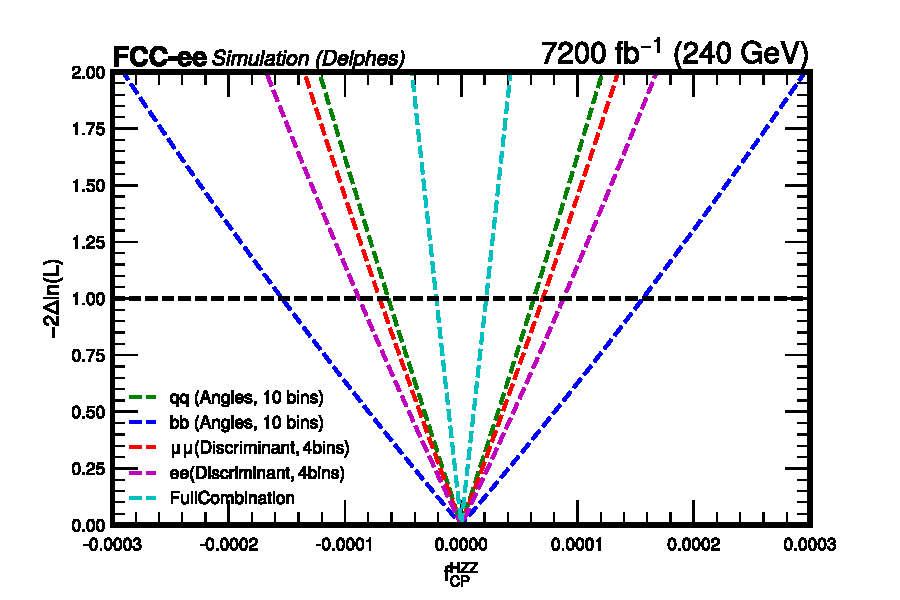
\includegraphics[width=0.7\linewidth]{full_7200_lumiscan.pdf}
    \caption{Likelihood scans for each individual channel as well as the combined result from all channels.}
    \label{fig:scan}
\end{figure}

 \Cref{fig:scan} shows the likelihood scans for $f^{\PH\PZ\PZ}_{CP}$ in each channel. 

 \begin{table}[]
     \centering
     \begin{tabular}{cc}
         Channel & $f^{\PH\PZ\PZ}_{CP}$ (68\% Confidence Limit) \\ \hline{}
          $\Pep\Pem$& $\pm 8.5*10^{-5}$ \\
          $\PGmp\PGmm$& $\pm 7.0*10^{-5}$\\
          $\PQb\PAQb$& $\pm 1.5*10^{-4}$\\
          $\PQq\PAQq$& $\pm 6.0*10^{-5}$\\
          Combination& $\pm 2.0*10^{-5}$\\
     \end{tabular}
     \caption{}
     \label{tab:my_label}
 \end{table}